%%%%%%%%%%%%%%%%%%%%%%%%%%%%%%%%%%%%%%%%%
% BAKALÁRSKÁ PRÁCE			%
% JAKUB FLAŠKA				%
% Šablona prevzata ze stránek KSE	%
% (C) FJFI CVUT v Praze			%
%%%%%%%%%%%%%%%%%%%%%%%%%%%%%%%%%%%%%%%%%

% Typ dokumentu
\documentclass[a4paper,12pt]{report}	% report - jednostranný tisk

%%%%%%%%%%%%%%%%%%%%%%%%%%%%%%%%%%%%%%%%%%%%%%%%%%%
%% Pouzite balícky

% Kódování a zpracování CJ
%\usepackage[czech]{babel}	% cestina
\usepackage[T1]{fontenc}	% balicek fontu
\usepackage[utf8]{inputenc}	% cestina
% Vytvorení indexu a seznamu použité literatury
\usepackage{index}		% vytvorení obsahu
\usepackage[pdftex]{hyperref}	% vygeneruje rejstrík pri použití pdflatex
\usepackage{cite}		% vytvorení literatury
\usepackage{multibib}		% více zdroju literatury
% Práce s obrázky
\usepackage{graphicx}		% obrázky
\usepackage{subfig}		% více obrázku v polícku
% Ostatní
\usepackage{listings}		% vkladani zdrojoveho kodu
\usepackage[usenames]{color}	% použití barevného textu
\usepackage{xcolor}
\usepackage{url}		% zpracování www adresy
\usepackage{verbatim}		% moznost viceradkovych kommentaru prikazem \begin{comment}
\usepackage{array}		%
\usepackage{caption}		% Popisky obrázku jiným písmem, než zbytek textu.
\usepackage{amsmath}
\usepackage[all]{hypcap}
\usepackage{caption}
\usepackage{pdfpages} 


%%%%%%%%%%%%%%%%%%%%%%%%%%%%%%%%%%%%%%%%%%%%%%%%%%%
%% Formát textu

\oddsidemargin=10mm		% levý okraj
\topmargin=-15mm		% horní okraj
\textwidth=150mm
\textheight=240mm
\pagenumbering{arabic}
\pagestyle{plain}

%\parindent=0pt			% odsazení prvního rádku
\parskip=7pt			% mezera mezi odstavci
\frenchspacing			% typografická pravidla

%\renewcommand{\rmdefault}{phv}	% Arial
%\renewcommand{\sfdefault}{phv}	% Arial


%%%%%%%%%%%%%%%%%%%%%%%%%%%%%%%%%%%%%%%%%%%%%%%%%%%
% Nastavení balícku
%%%%%%%%%%%%%%%%%%%%%%%%%%%%%%%%%%%%%%%%%%%%%%%%%%%


%%%%%%%%%%%%%%%%%%%%%%%%%%%%%%%%%%%%%%%%%%%%%%%%%%%%
%% Formátováni zdroju - cite, Multibib
%Bibtex
\bibliographystyle{./czechiso}		% styl primarnich zdroju

\newcites{sec}{Secondary Sources}	% sekundarni zdroje
\bibliographystylesec{./flaska}		% styl sekundarnich zdroju

%%%%%%%%%%%%%%%%%%%%%%%%%%%%%%%%%%%%%%%%%%%%%%%%%%%
% Vytvorení indexu pro rejstrík a citace - index
%index
\newindex{default}{idx}{ind}{}

%%%%%%%%%%%%%%%%%%%%%%%%%%%%%%%%%%%%%%%%%%%%%%%%%%%
%%%%%%%%%%%%%%%%%%%%%%%%%%%%%%%%%%%%%%%%%%%%%%%%%%%

\DeclareFontShape{OT1}{cmtt}{bx}{n}{cmttb10}{}	% Definování fontu pro bold type-writer.

% Caption
\captionsetup{%font=small,		% Formát popisku.
	format=plain,
	labelfont=bf,
	%textfont=it
}



% Nastavení odkazu - hyperref
\hypersetup{ 
linkbordercolor={1 1 1},	% rámecek kolem odkazu bude bílý
citebordercolor={1 1 1}		% rámecek kolem odkazu citace bude bílý 
} 

% Nastavení balícku pro vkládání zdrojového kódu - lstlistings
\definecolor{LightGray}{RGB}{245,245,245}
%\definecolor{LightRed}{RGB}{255,100,100}
%\definecolor{LightGreen}{RGB}{70,150,60}
%\definecolor{LightBlue}{RGB}{80,100,240}

\definecolor{LightRed}{RGB}{255,100,100}
\definecolor{LightGreen}{RGB}{60,143,49}
\definecolor{LightBlue}{RGB}{39,62,237}
\definecolor{Purple}{RGB}{162,4,207}

\newcommand{\red}[1]{\textcolor{red}{#1}}
\newcommand{\orange}[1]{\textcolor{orange}{#1}}
\newcommand{\lightgreen}[1]{\textcolor{LightGreen}{#1}}
\newcommand{\lightblue}[1]{\textcolor{LightBlue}{#1}}

\lstset{ %
language=C++,                % choose the language of the code
basicstyle=\small\tt\color{black},          % print whole listing small
keywordstyle=\small\color{LightBlue},	% bold black keywords
identifierstyle=\small\color{black},           % nothing happens
commentstyle=\small\color{black}, % white comments
stringstyle=\ttfamily,      % typewriter type for strings
showstringspaces=false,     % no special string spaces
numbers=left,                   % where to put the line-numbers
numberstyle=\tiny\tt,      % the size of the fonts that are used for the line-numbers
%stepnumber=2,                   % the step between two line-numbers. If it's 1 each line will be numbered
numbersep=5pt,                  % how far the line-numbers are from the code
%backgroundcolor=\color{LightGray},  % choose the background color. You must add \usepackage{color}
showspaces=false,               % show spaces adding particular underscores
showstringspaces=false,         % underline spaces within strings
showtabs=false,                 % show tabs within strings adding particular underscores
frame=single,			% adds a frame around the code
tabsize=3,	                % sets default tabsize to 2 spaces
%captionpos=b,                   % sets the caption-position to bottom
breaklines=true,                % sets automatic line breaking
breakatwhitespace=false,        % sets if automatic breaks should only happen at whitespace
%title={Zdrojovy kod},                 % show the filename of files included with \lstinputlisting; also try caption instead of title
%escapeinside={\%*}{*)}          % if you want to add a comment within your code
escapechar=!,
}

%\renewcommand{\lstlistingname}{Kód}


\renewcommand{\textfraction}{0.05}
\renewcommand{\topfraction}{0.2}	% max fraction of floats at top
\renewcommand{\bottomfraction}{0.2}	% max fraction of floats at bottom

%\setlength{\topsep}{10pt}
%\setlength{\itemsep}{10pt}

\newcommand{\redlist}[1]{{\color{LightRed}#1}}
\newcommand{\greenlist}[1]{{\color{LightGreen}#1}}

%%%%%%%%%%%%%%%%%%%%%%%%%%%%%%%%%%%%%%%%%%%%%%%%

% Formátování C++ príkazu uprostred textu
\newcommand{\clist}[1]{\texttt{\hyphenchar\font45\relax #1}} % font s fixní vzdáleností

% Makro pro ceské uvozovky, použití \uv{...}
\def\bq{\mbox{\kern.1ex\protect\raisebox{-1.3ex}[0pt][0pt]{''}\kern-.1ex}}
\def\eq{\mbox{\kern-.1ex``\kern.1ex}}
\def\ifundefined#1{\expandafter\ifx\csname#1\endcsname\relax }%
\ifundefined{uv}%
        \gdef\uv#1{\bq #1\eq}
\fi

\hyphenation{Open-GL}

%%%%%%%%%%%%%%%%%%%%%%%%%%%%%%%%%%%%%%%%%%%%%%%%%%%%%%
%%%%%%%%%%%%%%%%%%%%%% BAKALARSKA PRACE %%%%%%%%%%%%%%
%%%%%%%%%%%%%%%%%%%%%%%%%%%%%%%%%%%%%%%%%%%%%%%%%%%%%%

%%%%%%%%%%%%%%%%%%%%%%%%%%%%%%%%%%%%%%%%%%%%%%%%%%%%
%%%%%%%%%%%%%%%%%%%%%% POJMY  %%%%%%%%%%%%%%%%%%%%%%            

\newcommand{\cvut}{Czech Technical University in Prague}
\newcommand{\fjfi}{Faculty of Nuclear Sciences and Physical Engineering}
\newcommand{\km}{Department of Mathematics}
\newcommand{\obor}{Inženýrská informatika}
\newcommand{\zamereni}{Tvorba software}
\newcommand{\nazevcz}{Softwarový nástroj pro manipulaci s daty z magnetické rezonance a jejich vizalizaci}
\newcommand{\nazeven}{Development of a Software Instrument for MRI Data Manipulation and Visualization }     
\newcommand{\autor}{Bc.~Jakub Flaška}
\newcommand{\rok}{2012}
\newcommand{\vedouci}{Ing.~Pavel Strachota} 

%%%%%%%%%%%%%%%%%%%%%%%%%%%%%%%%%%%%%%%%%%%%%%%%

%%%%%%%%%%%%%%%%%%%%%% UVODNI STRANA  %%%%%%%%%%%%%%%%%%%%%%

\begin{document}

\includepdf[pages=-]{Uvod/uvod.pdf} 

%%%%%%%%%%%%%%%%%%%%%% OBSAH %%%%%%%%%%%%%%%%%%%%%%
\newpage
\tableofcontents


%\begin{comment}
%%%%%%%%%%%%%%%%%%%%%% PROSTOR PRO ZADANI  %%%%%%%%%%%%%%%%%%%%%%
\newpage
\thispagestyle{empty} 

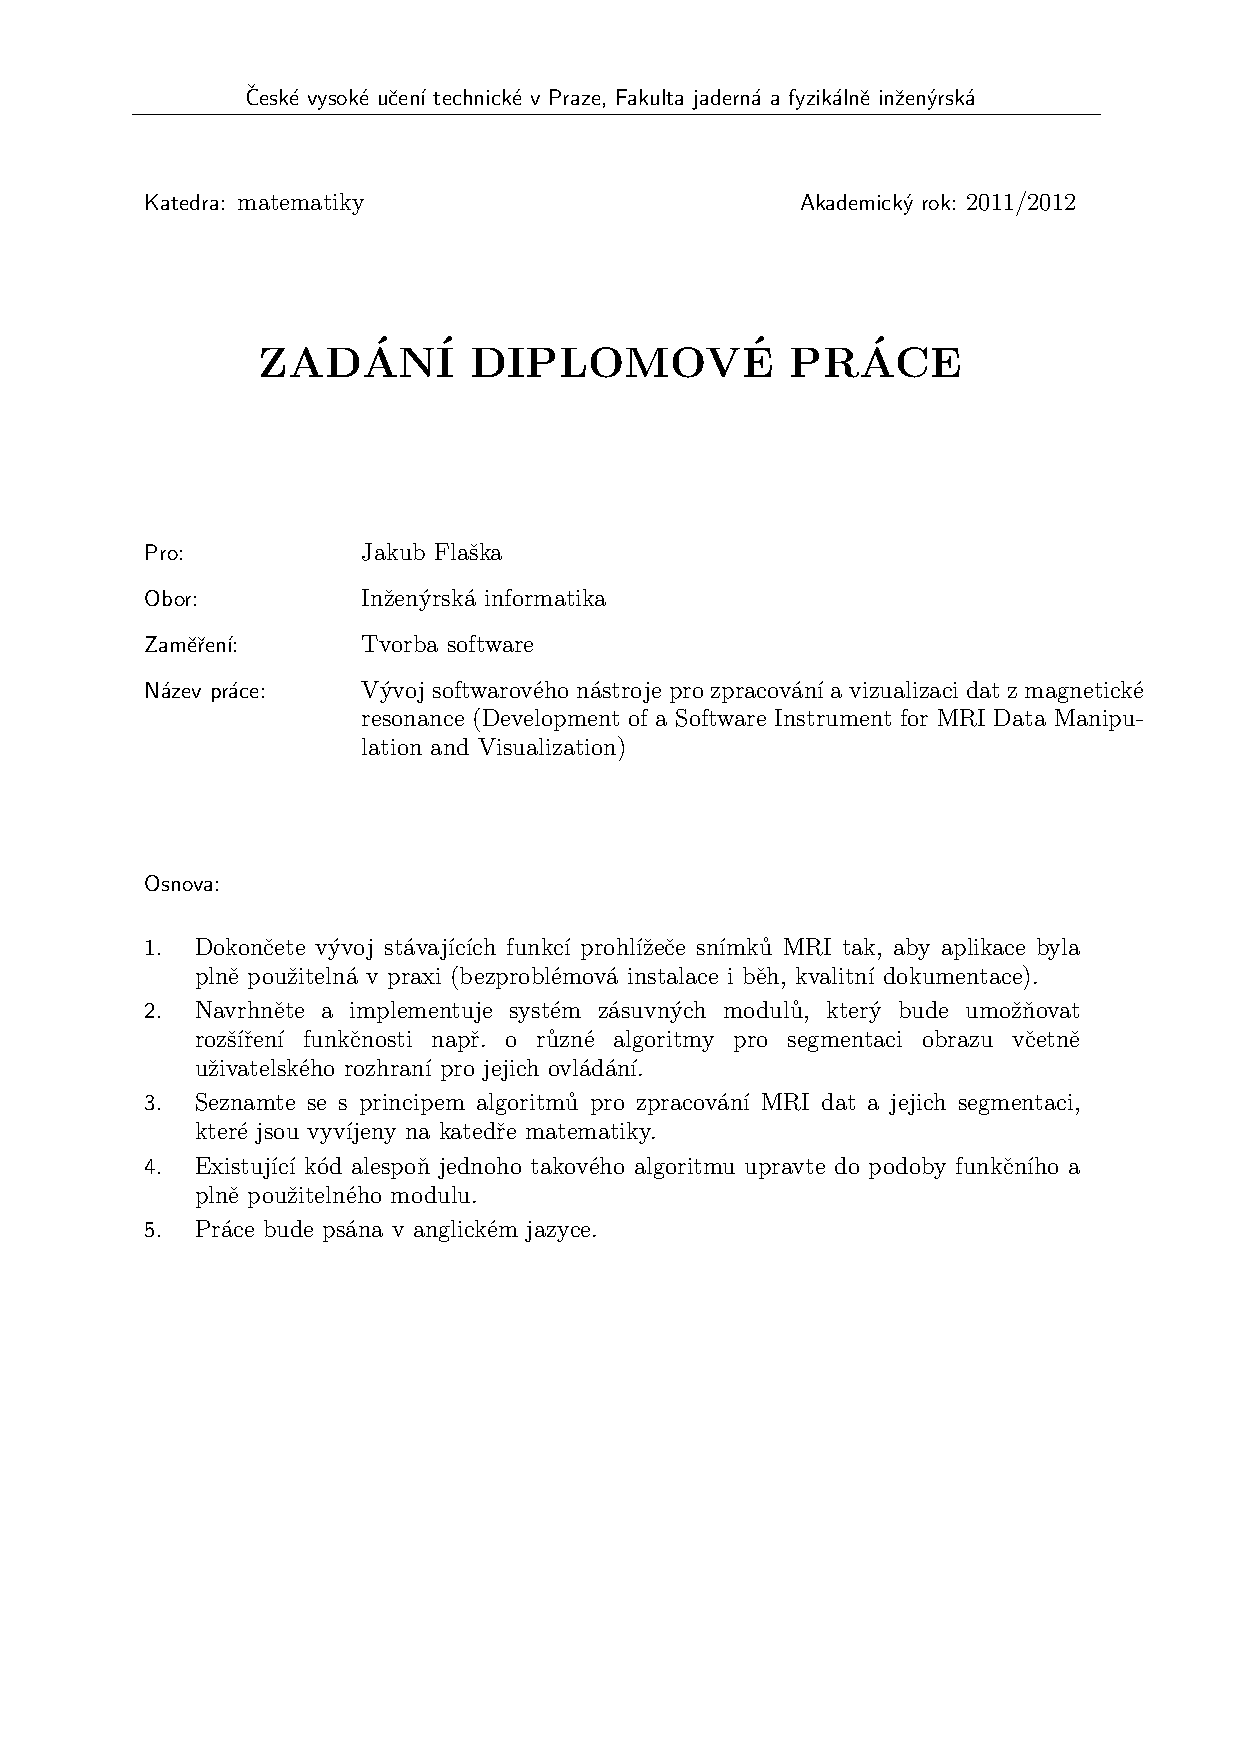
\includepdf[pages=-]{Text/IMG/zadani.pdf} 

%%%%%%%%%%%%%%%%%%%%%% PROHLASENI %%%%%%%%%%%%%%%%%%%%%%
\newpage
\thispagestyle{empty}

~
\vfill % prázdné místo

{\bf Author's Statement}

\vspace{0.5cm} % vertikální mezera

Hereby, I certify that this diploma thesis is my own work. I have not assumed any of the texts, all the text are written by my person. 

I am not against using this diploma thesis by Czech Technical University in any way described in ``Zakon autorsky'' about school projects.

Noone except the author and Czech Technical University has a right to manipulate with the text - noone can copy the text or part of the text and use it in another work.

I am not against redistributing the whole text - if the text will be distributet together with the initial page and its autorship will be clear.

\vspace{10mm}

Tímto prohlašuji, že tato diplomová práce je mým autorským dílem. Texty v práci nejsou prevzaté, ale jsou psané autorem.

Nemám závažný duvod proti použití tohoto díla Ceským Vysokým Ucením Technickým tak, jak to vyplívá z autorského zákona v textu o školním díle. 

Kdokoliv mimo autora a Ceské Vysoké Ucení Technické pak nemá právo s textem manipulovat - zejména pak celý text, nebo cást textu vydávat za autorské dílo nekoho jiného.

Umožnuji pak šírení kompletního textu této diplomové práce, pokud bude text šíren jako celek vcetne úvodní strany a nebude pochybnost o jeho autorství. 

\vspace{10mm}Praha, June 5, 2012\hfill
	\begin{tabular}{c}
	
\includegraphics[width=50mm]{Text/IMG/podpis.jpg}\\ 
	\autor
	\end{tabular}


%%%%%%%%%%%%%%%%%%%%%% PODEKOVANI %%%%%%%%%%%%%%%%%%%%%%
%\end{comment}
%\begin{comment}%%%%%%%%%%%%
\newpage
\thispagestyle{empty}

~
\vfill % prázdné místo

{\bf Acknowledgment / Podekování}

\vspace{5mm} % vertikální mezera

I would really like to thank my supervisor Ing. Pavel Strachota for his outstanding help while creating this diploma thesis. His suggestions greatly improved the text.

Rád bych podekoval svému školiteli Ing. Pavlu Strachotovi za vedení této diplomové práce. Jeho pripomínky byly znacne podnetné a výrazne prispely ke zkvalitnení textu.

\begin{flushright}
Author
\end{flushright}


%%%%%%%%%%%%%%%%%%%%%% ABSTRAKT %%%%%%%%%%%%%%%%%
%\end{comment}%%%%%%%%%%%
\begin{comment}
\newpage
\thispagestyle{empty}

% příprava:\usepackage{subfig}
\newbox\odstavecbox
\newlength\vyskaodstavce
\newcommand\odstavec[2]{
    \setbox\odstavecbox=\hbox{
         \parbox[t]{#1}{#2\vrule width 0pt depth 4pt}}
    \global\vyskaodstavce=\dp\odstavecbox
    \box\odstavecbox}
\newcommand{\delka}{120mm}


\newcommand{\pracovisteVed}{\km,\\ \fjfi,\\ \cvut}

\newcommand{\konzultant}{}
\newcommand{\pracovisteKonz}{}

\newcommand{\klicova}{programování, GUI, grafické uživatelské rozhraní, C++, Qt, DICOM}
\newcommand{\keywords}{programming, GUI, graphic user interface, C++, Qt, DICOM}   



{\noindent \bf \large Abstract} \\[5mm]
\begin{tabular}{l p{10cm}}
	{\em Master's Thesis}	& 	\\[1mm]
	{\em Title:}	& \nazeven	\\[1mm]
	{\em Author:}	& \autor	\\[1mm]
	{\em Program:} 	& \obor		\\[1mm]
	{\em Supervisor:}& \vedouci	\\
				& \km		\\
				& \fjfi		\\
				& \cvut		\\[1mm]
	{\em Keywords:}	& \odstavec{\delka}{\keywords}	\\
\end{tabular}

This Diploma Thesis describes development of a C++ application, which is used for displaying images caputured on Magnetic Resonance Imaging unit. Prior to this work, the application was partly implemented. This work sets a few goals: redesign the rendering part of the application, implement Multi-planar recontruction and a system for additional plugins. In addition, the thesis focuses on GUI applications programming and compilation of C++ applications in Win32.


\vspace{10mm}
{\noindent \bf \large Abstrakt} \\[5mm]
\begin{tabular}{l p{10cm}}
	{\em Diplomová práce}	& 	\\[1mm]
	{\em Název:}	& \nazevcz	\\[1mm]
	{\em Autor:}	& \autor	\\[1mm]
	{\em Keywords:}	& \odstavec{\delka}{\klicova}	\\
\end{tabular}

Tato diplomová práce se zabývá vývojem programu sloužícího pro zobrazování snímků z magnetické resonance. Na začátku této práce již byla aplikace částečně implementována. Tato diplomová práce se snaží zejména o následující úkoly: kompletně přepsat část aplikace věnující se vykreslování; implementovan systém zobrazení označovaný jako multiplanární rekonstrukce; přidat do aplikace rozhraní umožňující používání přídavných modulů k aplikaci. Dále se pak práce věnuje v obecnější rovině programování aplikací s grafickým uživatelským rozhraním a shrnuje poznatky o překladu C++ aplikací v prostředí Win32.






\end{comment}


%%%%%%%%%%%%%%%%%%%%%%  TEXT PRÁCE %%%%%%%%%%%%%%%%%%%%%%%%%%%%%%%%%%%%%%%%%%%%

\chapter{Introduction}
\vspace{-10mm}
The aim of this Diploma Thesis is development of a C++ application used for viewing Magnetic Resonance data. The task was given by IKEM institute\footnote{Institute for Clinical and Experimental Medicine \cite{ikem}} and was started in work \cite{neskudla} and followed in works \cite{flaska_bc} and \cite{flaska_vu}. The application (further called ``Dicom-Presenter'') allows to open MRI images and offers unique displaying features required by IKEM.

This Diploma Thesis sets three goals to be done: handle project compilation, rewrite application rendering engine and implement new features. The project compilation process needed to be reviewed and automated. There were dependencies on five external libraries which complicated project deployment. Therefore, the rendering part of the application had to be rewritten to remove project dependency on 3rd party libraries like OpenGL\citesec{openglhome}, Cg toolkit\citesec{cgtoolkit}, plib\citesec{plibhome}. Lastly, multi-planar reconstruction\footnote{A multi-planar reconstruction is a way for displaying three-dimensional images. Three slices in three perpendicular planes are displayed. See Chapter \ref{multiplanar}.} and image segmentation were added into the application.



\chapter*{Dicom-Presenter}
\addcontentsline{toc}{chapter}{Dicom-Presenter}
\vspace{-10mm}

My predecessor Bc. Pavel Neskudla started development of an application for viewing images from MRI as a part of his master's thesis\cite{neskudla}. It was a task given by IKEM institute in Prague\footnote{Institute for Clinical and Experimental Medicine}. IKEM institute specialists found out that they would utilize some application which would allow them to open MRI images elsewhere than only on Siemens computers located in their institute. They would prefer some application where they could view recorded images on their own personal computers. It is possible to find such applications distributed by local developers, but only a few of them reach satisfactory quality requirements. These are definitely commercial applications, so user has to pay. There is also a lot of non-commercial, freeware applications, but functionality of these applications is often limited\cite[page~9]{flaska_bc}. For example, it was not possible to find an application which could open several images at the same time and view them on one screen. Therefore, specialists from IKEM institute decided to ask our faculty to develop such an application which would fit their needs.

\begin{figure}
	\begin{center}
	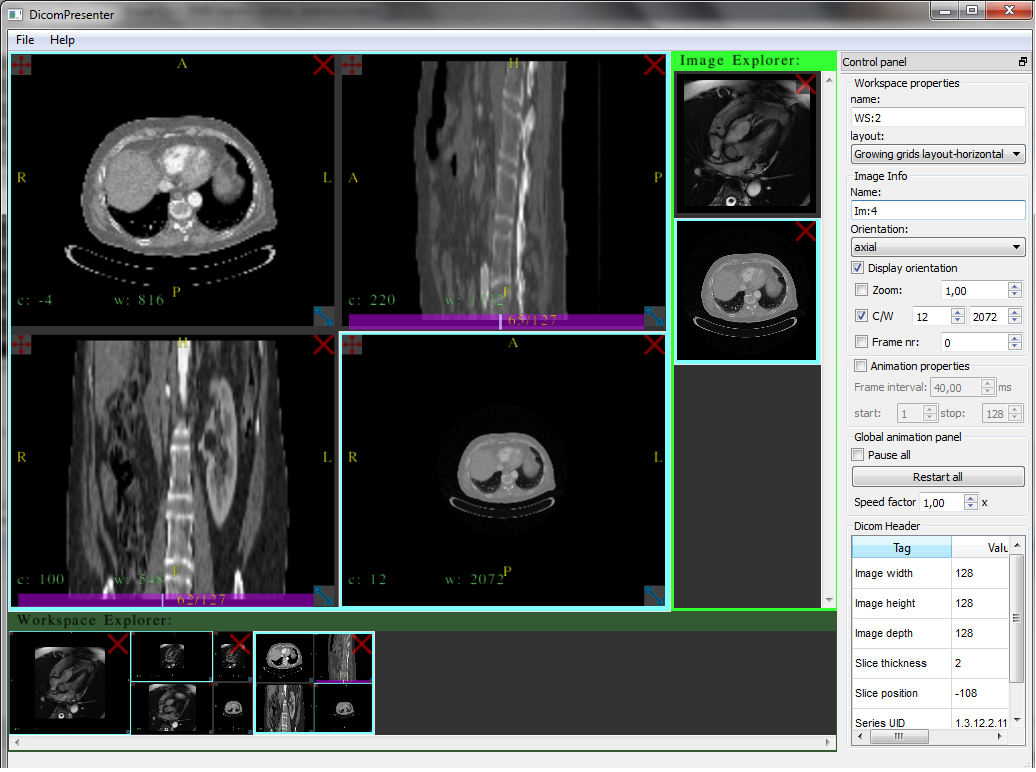
\includegraphics[width=130mm]{Text/IMG/04_GUI_Screenshot.png}
	\end{center}
	\caption{Screenshot of Dicom-Presenter user interface.}
	\label{screenshot}
\end{figure}

\section*{Application requirements}
\addcontentsline{toc}{section}{Application requirements}
The IKEM specialists asked for a typical DICOM images viewer with few more specific features which they missed in freeware programs. A typical DICOM viewer allows you to open .dcm files and display it. .dcm file in this case is a jpeg image equipped with special header including patient's information. There you can see a 2D picture of some part of the patient's body. Some DICOM viewers allow you to open series of .dcm files, which can actually fit into a three-dimensional picture. Less commonly it can be a time animation of organ behaviour in short time period (f.e. one heart beat). DICOM viewers often have some more functions but it is very individual.

There have been two more specific requirements on application functionality by IKEM specialists. They missed certain functions in freeware DICOM applications. The most important function was a possibility to open several images at one time and display them on one screen. The user should be allowed to arrange images on screen to any possible layout he prefers. This functionality allows physicians to see two or more different MRI images on screen so they can easily determine pathological differences among observed organs. It is useful for studying, or teaching.

There have been also requirements that the application should be able to record user's manipulation with images as a video. Then physician can prepare his presentation of images at home and then play the video in front of crowds.

\begin{table}[ht]
	\caption{DICOM viewers.}
	\centering
	\begin{tabular}{cc}
			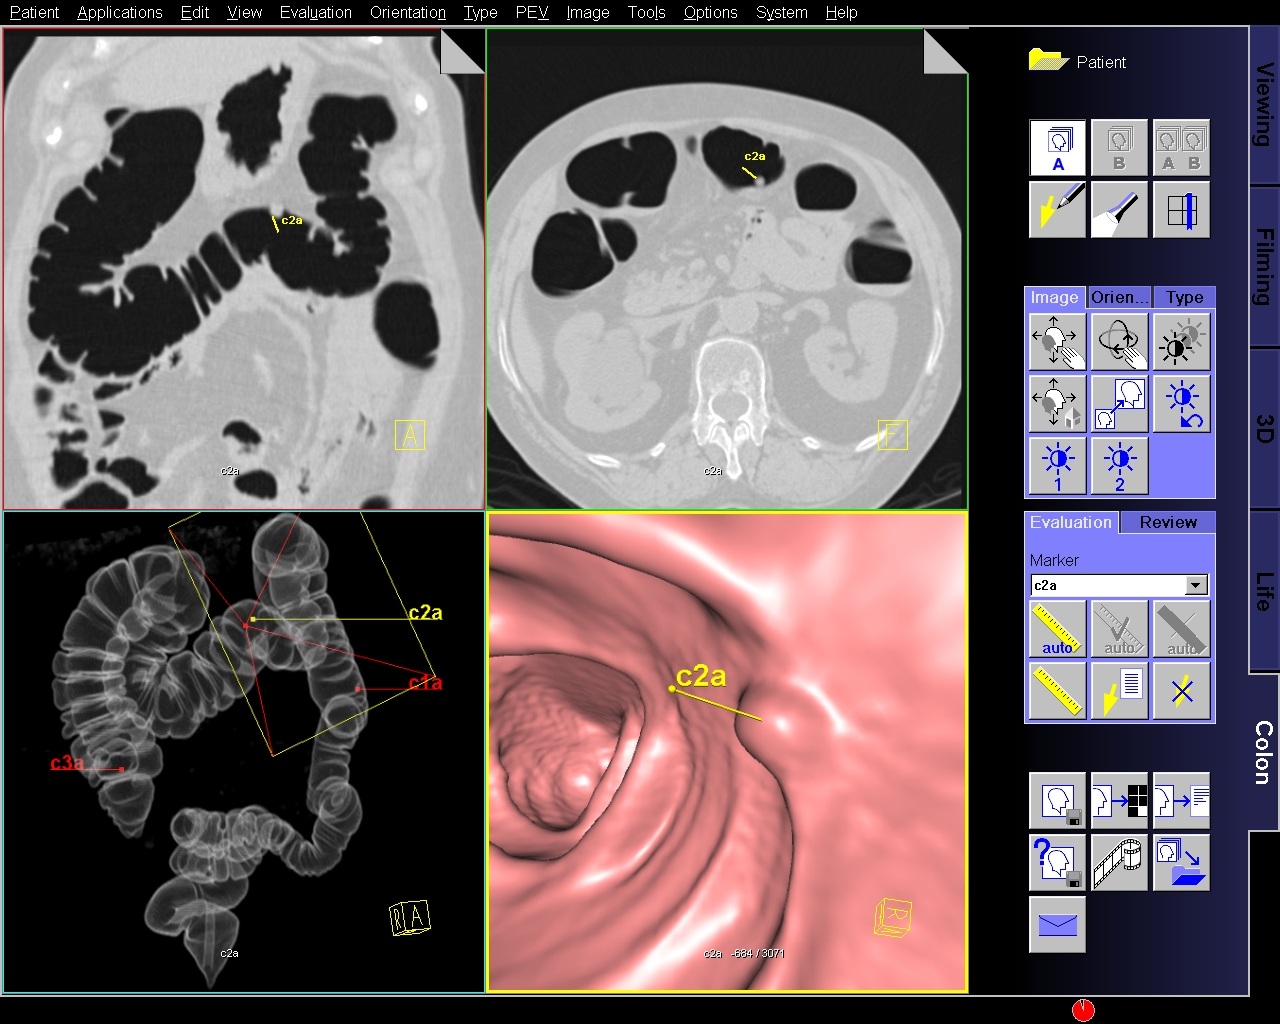
\includegraphics[width=0.5\textwidth,height=0.375\textwidth]{Text/IMG/01_Siemens.jpg}
		&
			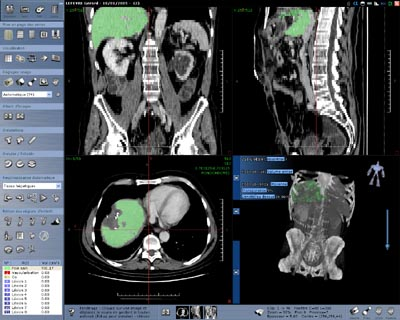
\includegraphics[width=0.5\textwidth,height=0.375\textwidth]{Text/IMG/01_Myrian.jpg}
		\\
			syngo Imaging~\citesec{siemens} & Myrian~\citesec{intrasense}	
		\\
			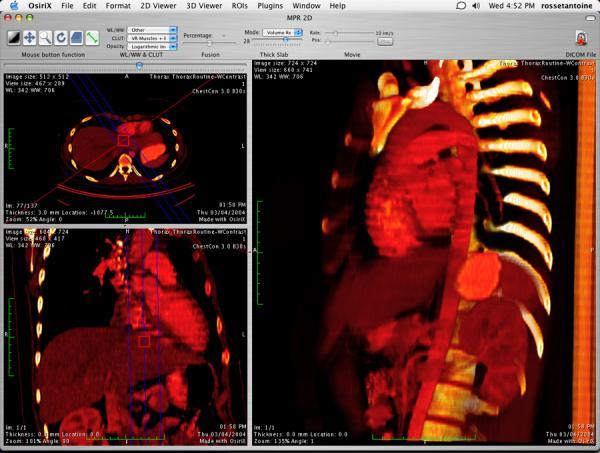
\includegraphics[width=0.5\textwidth,height=0.375\textwidth]{Text/IMG/01_OsiriX.jpg}
		&
			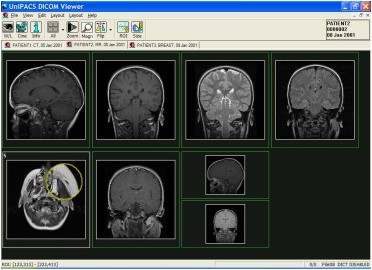
\includegraphics[width=0.5\textwidth,height=0.375\textwidth]{Text/IMG/01_UniPACS.jpg}
		\\
			OsiriX~\citesec{osirix} & UniPACS~\citesec{unipacs}
		\\
		\end{tabular}
\end{table}%

\section*{Application functionality}
\addcontentsline{toc}{section}{Application functionality}
\chapter{Graphic User Interface Programming}
\vspace{-10mm}

A Graphic User Interface (GUI) of an application has to be described in its source code - control elements' layout and their interaction. Each operation system offers its own library for GUI programming. To ease the programming process, additional libraries can be used - libraries, which are focused mainly on creating application's GUI are called Widget Toolkits.

The native libraries for GUI programming are for example Windows API in Windows and xlib in Linux/Unix systems. The process of programming application's GUI with use of only native OS library is following text explained on Windows API. Object-oriented GUI programming is explained with use of Qt\citesec{qthome} and GTK\citesec{qthome} libraries.

\section{GUI programming in Windows API library}
\label{noqt}
Creating an application's GUI with use of only OS related library is quite complicated. The native libraries are simple - both Windows API and xlib are not object-oriented. The application behavior has to be solved by procedural declarations in the source code.

The GUI programming in WinAPI uses following basic elements\cite[Chapter~2]{eventloopprogramming}:

\begin{itemize}
\item Object
\item Object's Procedure
\item Message
\item Message Queue
\item Message Loop
\end{itemize}

The basic idea is following:

\begin{itemize}
\item The core of the application is the Message Loop. It loads messages from the Message Queue and redirects them to proper Objects.
\item Each Object owns a Procedure. The Procedure receives a message and adds the response to Message Queue.
\end{itemize}

This concept is called event-driven programming. There is an example of event-driven application on Listing \ref{WinAPI}. The application loop is located on line \ref{lst:ProgramLoop}. The \clist{GetMessage} functions reads a message from the Message Queue. The \clist{DispatchMessage} forwards the message to propriate object.

The only visible object of the example application is a window created on line \ref{lst:window}. The procedure of the window, which solves its received messages is defined on line \ref{lst:WndProc}.

The \clist{main} function of the application is replaced by the \clist{WinMain} function. So the application course is following: the window is created and the loop starts running; if the user clicks on the window, a message is added to the queue; the message is readed from the queue and then forwarded to the application itself or back to the window.\cite[Chapter~2]{eventloopprogramming}

\begin{lstlisting}[label=WinAPI,caption={An example of a simple application using Windows API for GUI rendering.\protect\cite{WinAPIexample}},escapeinside={@}{@}]
@\label{lst:WndProc}@LRESULT CALLBACK WndProc(HWND hwnd, UINT msg, WPARAM wParam, LPARAM lParam){
    switch(msg){
        case WM_CLOSE:
            DestroyWindow(hwnd);
        break;
        case WM_DESTROY:
            PostQuitMessage(0);
        break;
        default:
            return DefWindowProc(hwnd, msg, wParam, lParam);
    }
    return 0;
}
@\label{lst:WinMain}@int WINAPI WinMain(HINSTANCE hInstance, HINSTANCE hPrevInstance,
    LPSTR lpCmdLine, int nCmdShow){
    WNDCLASSEX wc;
    HWND hwnd;
    MSG Msg;
    //Step 1: Registering the Window Class
    wc.cbSize        = sizeof(WNDCLASSEX);
    wc.style         = 0;
    wc.lpfnWndProc   = WndProc;
    wc.cbClsExtra    = 0;
    wc.cbWndExtra    = 0;
    wc.hInstance     = hInstance;
    wc.hIcon         = LoadIcon(NULL, IDI_APPLICATION);
    wc.hCursor       = LoadCursor(NULL, IDC_ARROW);
    wc.hbrBackground = (HBRUSH)(COLOR_WINDOW+1);
    wc.lpszMenuName  = NULL;
    wc.lpszClassName = g_szClassName;
    wc.hIconSm       = LoadIcon(NULL, IDI_APPLICATION);
    // Step 2: Creating the Window
 @\label{lst:window}@   hwnd = CreateWindowEx(
        WS_EX_CLIENTEDGE,
        g_szClassName,
        "The title of my window",
        WS_OVERLAPPEDWINDOW,
        CW_USEDEFAULT, CW_USEDEFAULT, 240, 120,
        NULL, NULL, hInstance, NULL);
    // Step 3: The Message Loop
@\label{lst:ProgramLoop}@    while(GetMessage(&Msg, NULL, 0, 0) > 0){
        TranslateMessage(&Msg);
        DispatchMessage(&Msg);
    }
    return Msg.wParam;
}
\end{lstlisting}

Programming GUI applications in plain WinAPI requires necessary steps to be done, such as: defining the main loop, assigning a procedure to the object, etc. All these steps are ensured by Widget Toolkits, if used. 

\begin{comment}

\section{GUI programming in Windows API}
Development of GUI application for Windows is possible with Windows API. This is the name given to a set of various APIs - communication interfaces for performing services. These communication interfaces offer manipulation with file-system, devices and also creating graphic windows.

Most common parts of Windows API are:
\begin{itemize}
\item \clist{kernel32.dll}, which is needed for memory management, input/output, process and thread creation.
\item \clist{user32.dll} for creating GUI elements, such as windows, buttons, etc.
\item \clist{shell32.dll} which offers access to Windows command line
\item \clist{WinSock} to use network
\end{itemize}
\end{comment}

\section{Widgets Toolkits}
\label{guiframeworks}
Widgets Toolkits are libraries designed to ease GUI application creation. Complicated widget declaration processes are encapsulated inside the library. Then, library classes are used instead of calling OS related functions. Examples of currently popular Widgets Toolkits can be Qt\citesec{qthome} and GTK\citesec{gtkhome} libraries\cite[pages~413-416]{qtvsgtk}.

Both Qt and GTK are based on the same schema. All control elements are represented by library classes. The control elements can be easily added to application windows. Control functions describing application response to user actions are defined. Then the control elements and control functions are connected together.

Source code syntax of Qt library and GTK library is very similar. Examples of two identical applications using GTK and Qt can be found on Listings \ref{gtk} and \ref{qt}. Both applications create a simple window with a button inside. Clicking the button writes a console output. The button and window creation can be found on lines \ref{lst:gtkbuttonstart} - \ref{lst:gtkbuttonfinish} on Listing \ref{gtk} (GTK) and lines \ref{lst:qtbuttonstart} - \ref{lst:qtbuttonfinish} on Listing \ref{qt} (Qt). The process is very similar unlike Qt uses functions in its classes and GTK uses global functions. The command on lines \ref{lst:gtkconnect} (Listing \ref{gtk}) and \ref{lst:qtconnect} (Listing \ref{qt}) is used for setting up interaction between button click and proper function call. The main difference is that GTK allows connection to global function calls (line \ref{lst:gtkcall}, Listing \ref{gtk}), unlike Qt allows calling functions of object inheriting QObject class (line \ref{lst:gtkcall}, Listing \ref{qt}).

\begin{lstlisting}[label=gtk,caption={A sample application using GTK library.\protect\cite{gtktutorial}},escapeinside={@}{@}]
@\label{lst:gtkcall}@static void message(GtkWidget *widget, gpointer data){
    cout << "Hello World!";
}
...
@\label{lst:gtkbuttonstart}@GtkWidget *window = gtk_window_new (GTK_WINDOW_TOPLEVEL);
GtkWidget *button = gtk_button_new_with_label ("Hello World");
GtkWidget *layout = gtk_fixed_new();
gtk_fixed_put(GTK_FIXED(layout), button);
@\label{lst:gtkbuttonfinish}@gtk_container_add(GTK_CONTAINER(window), layout);
@\label{lst:gtkconnect}@g_signal_connect (button, "clicked", G_CALLBACK (message), NULL);
\end{lstlisting}

\begin{lstlisting}[label=qt,caption={A sample application using Qt library.},escapeinside={@}{@}]
@\label{lst:qtcall}@class callhandler : public QObject {
Q_OBJECT
public slots:
	void message () {
		cout << "Hello World!";
	}
}
...
@\label{lst:qtbuttonstart}@QWidget *window = new QWidget();
QPushButton *button = new QPushButton();
QLayout *layout = new QGridLayout();
layout->add(button);
@\label{lst:qtbuttonfinish}@window->setLayout(layout);
@\label{lst:qtconnect}@connect(button,SIGNAL(clicked()),callhandler,SLOT(message()));
\end{lstlisting}
\chapter{Image manipulation}
\vspace{-10mm}

Dicom-Presenter is an application for viewing image data. Entire image manipulation was solved with use of OpenGL library in early version of Dicom-Presenter. OpenGL was used for image storing, for changing image properties and for drawing images on screen. Unfortunately, OpenGL brought complications to application compatibility with various hardware. Therefore, author of this work decided to remove OpenGL from application and replace all classes using OpenGL with their non-OpenGL equivalents. 

Before rewriting all image processing classes without OpenGL it was a need to study how to complete all image processing tasks without OpenGL. Moreover, OpenGL uses GPU to perform its tasks so it was a need to calculate the loss of performance when OpenGL will be removed. 

\section{Image storing}
\label{rawdata}
There are two different libraries used for image manipulation in Dicom-Presenter. DCMTK library is used for loading images from hard disk, while Qt library (formerly OpenGL) is used for displaying images on computer screen. DCMTK library must be used since it supports loading files in DICOM format, moreover some application framework must be used for image displaying. DCMTK library offers loading compressed image files and saving them uncompressed into RAM memory. To be able to display these raw data properly by Qt library, it is mandatory to understand the way image data are represented in computer. 

A color image consisting of $m \cdot n$ points (pixels) can be described by $m \cdot n$ number triads. The triads would be coordinates in RGB or HSV color space \footnote{Colors which can be displayed can be fully described by three values. This fact is based on human eye anatomy and leads to construction of coordinate systems describing each displayable color. Coordinates of RGB color space are red, blue, green color while hue, saturation, value are coordinates in HSV color space.}. Data in a computer are stored in elementary units - bytes, which can hold 256 different values. Each byte consists of eight unitary units - bits ($2^8 = 256 $). If considered that one byte can include color information of only one pixel, then only eight-bit multiples can be used for a pixel color storage: 8 bits, 16 bits, 24 bits, etc. In case of 24 bit color depth, three bytes are used for a pixel color storage - each byte for each color. If 8 bits depth or 16 bits depth is used, in both cases the bit numbers are not divisible by three, so there are several ways of how to distribute bits among colors.
 
Qt library uses three different formats of 16 bit color information storage. The formats differ by number of bits distributed to each color and are described by triads of numbers: 5-6-5, 5-5-5, 4-4-4. The first format uses 5 bits for red color, 6 bits for green color and 5 bits for blue color. The numbers of bits for each color are uneven but no redundant bits are present. Both 5-5-5 and 4-4-4 formats include redundant bits for each image pixel.

Qt library allows displaying images which are actually saved in computer memory as an array of bytes in some of supported formats (such as described above). Next to color depth formats, image storage can differ by number of bytes used for storing each image line. If an image has $m \cdot n$ pixels and two bytes are used per pixel (f.e. 16 bit 5-5-5), there is no rule that $m \cdot n \cdot 2$ bytes will be used. A computer memory in x86 architecture reads its data in elements called words usually consisting of 4 bytes for x86 architecture and 8 bytes for 64-bit architecture. Therefore, image data are in computer memory often aligned that each image line starts at a beginning of some 4-byte or 8-byte word. For instance, if we consider an image of $100 \cdot 100$ pixels saved with 8 bit pixel depth on 64-bit architecture, each line consisting of $100$ pixels would be saved on $128$ or bytes.

In conclusion, if a picture is reconstructed from uncompressed raw data saved in computer memory, essential indications are which color storage format is used for each pixel and which bit align is used for each pixel-line. Those two information are enough for correct image reconstruction.

\subsection{Image construction from raw data in Qt library}
As said in previous text, DCMTK library allows loading compressed files from hard disk and saves them into RAM memory in one of mentioned data alignment. Qt library allows displaying the image data onto computer screen. It is mandatory to coordinate an output of DCMTK and an input of Qt library to be able to display an image properly.

DCMTK library offers a function which saves a copy of loaded image data into a new place in image memory in required data alignment. The function declaration is:

\clist{const void* DicomImage::getOutputData	(const int bits = 0,
const unsigned long frame = 0,
const int planar = 0 )}

The first parameter denotes a required data alignment of each pixel; the other two parameters describe the orientation of the image slice inside the three-dimensional texture. The function returns a pointer to the part of memory where image data will be stored.

Besides, Qt library offers a construction of its object depending on image data already stored in computer memory. The object receives a pointer to image data through its constructor. If the image data meet prospective requirements, the object can be called to draw the image at any time, as long as the data are still on the place in computer memory.

The constructor declaration is:

\clist{QImage::QImage(uchar* data, int width, int height, int bytesPerLine, Format format)}

The first parameter is a pointer to image data already saved in computer memory. The data are declared as \clist{unsigned char} which is a C++ equivalent of a \clist{byte} type. The last parameter \clist{format} describes a pixel alignment. It describes a number of bytes used for each pixel and a particular way of color information storage. The \clist{bytesPerLine} parameter describes an image line alignment of pixel data.

Qt library itself cannot determine the exact values of above described parameters. Therefore, the parameter values must be known before. A misleading value of parameter describing pixel color storage will lead to false color interpretation of the image. Furthermore, incorrect parameter describing image line alignment can avert image loading or can cause a program failure due to unauthorized memory access.  


\begin{figure}
	\begin{center}
	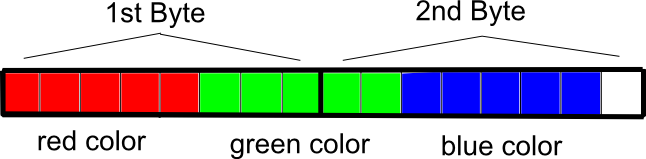
\includegraphics[width=130mm]{Text/IMG/ImageStoring_16bit.png}
	\end{center}
	\caption{A distribution of 16 bits of 2 bytes among three colors of a pixel.}
	\label{imagestoring}
\end{figure}

\section{Image enhancement operations}
\label{brightnesscontrast}

One of important tasks to re-implement in Dicom-Presenter was an ability to adjust image brightness and contrast. Images which will be opened in Dicom-Presenter can be captured on various MRI units with various imaging properties. The ability to increase image brightness and contrast is mandatory to ensure sufficient display quality. Too dark or too gray images need to be brightened or need to increase contrast to ensure better observation of physiological findings. A brightness and contrast change is among DICOM users called ``windowing''.

For further needs of this text brightness and contrast need to be defined. 

A gray-scale image can be considered as a matrix of numbers: 

\[
 Im_{res_{x},res_{y}} =
 \begin{pmatrix}
  Im(1,1) & Im(1,2) & \cdots & Im(1,res_{x}) \\
  Im(2,1) & Im(2,2) & \cdots & Im(2,res_{x}) \\
  \vdots  & \vdots  & \ddots & \vdots  \\
  Im(res_{y},1) & Im(res_{y},2) & \cdots & Im(res_{y},res_{x})
 \end{pmatrix}
\]

where $ res_{x} $, $res_{y}$ are dimensions of the image. $Im(x,y)$ is a lightness of a pixel.

Brightness then can be defined as:
\[
  Brightness(Im) = \frac{1}{res_{x}  \cdot res_{y}}\sum_{\substack{0 \leq x \leq res_{x} \\ 0 \leq y \leq res_{y}}} Im(x,y)
\]

Contrast is understood as overall difference in luminosity between bright and dark pixels. There are more possible definitions of contrast. One possible definition is:

\[
Contrast(Im) = \sqrt{\frac{1}{res_{x} \cdot res_{y}}\sum_{\substack{ 0 \leq x \leq res_{x} \\ 0 \leq y \leq res_{y} }}(Im_{x,y}-Brightness(Im))^2}
\]

An argument for using these two definitions for brightness and contrast is that they are analogies for mean value and variance of set of values.

If there is a need of increasing or decreasing image brightness in computer applications simply a constant is added to all image points:

\begin{equation}
\label{brightness}
  Im(x,y) \longmapsto Im(x,y) + c_{brightness} 
\end{equation}

Image contrast is usually adjusted by a linear transformation applied to all image points:

\begin{equation}
\label{contrast}
  Im(x,y) \longmapsto   (Im(x,y) - 0.5) \cdot c_{contrast} + 0.5
\end{equation}

A disadvantage of both ways is that some image information is lost. Let's consider an image described by a matrix with elements of integers in range from zero to 255. Let the brightness of the picture increased according to formula \eqref{brightness} with a positive constant $ c_{brightness} $. Then all the points brighter than $ 255 - c_{brightness} $ on original image will have luminosity of 255 regardless their original luminosity. Similarly if contrast would be increased according to formula \eqref{contrast} with a constant $ c_{contrast} $ then all points brighter than $ \frac{1}{2} \cdot 255 \cdot (\frac{1}{c_{contrast}}+1) $ will have the same color (maximum white). As well all pixels darker than $ \frac{1}{2} \cdot 255 \cdot (1 - \frac{1}{c_{contrast}}) $ will have the same color (maximum black).

\clist{krivka na nelinearni kontrast z vyzkumaku}

\subsection{Pixel manipulations in Qt}

Qt library doesn't offer its own functions for elementary pixel manipulations such as change of brightness and contrast. These operations (described in Section \ref{brightnesscontrast}) must be done in application source code for each image pixel.

A change of brightness or contrast of an image of $m \cdot n$ pixels will be done in $m \cdot n$ steps. In each step a color of the pixel must be obtained, new color value will be calculated and the value will be saved into the picture. Qt library offers two ways to perform the task: pixel manipulation functions or direct memory access.

If pre-implemented Qt pixel manipulation functions are used, the source code will be following:

\begin{lstlisting}[label=qtcontrast,caption={Image enhancement operations implementation using Qt library functions for pixel manipulation.},escapeinside={@}{@}]
QImage image(...);
for (int y=0; y<height; y++) {
	for (int x=0; x<width; x++) {
		@\label{lst:pixel}@QRgb color = image.pixel(x,y);
		@\label{lst:operation}@QRgb newcolor = qRgb(func1(qRed(color)),func2(qGreen(color)),func3(qBlue(color)));
		@\label{lst:setPixel}@image.setPixel(x,y,color);
	}
}
\end{lstlisting}

Function \clist{QRgb QImage::pixel(int x,int y)} is used to retrieve color information of a pixel. The code on line \ref{lst:operation} performs a color manipulation. Function \clist{void QImage::setPixel(int x,int y,QRgb rgb)} is used to save the color information back to the picture. Due to multi-thread programming support the \clist{QImage::setPixel} function offers low performance. Within each function call Qt library must attach and detach a process to shared memory segment where the image data are stored. These steps are performance expensive.

Nevertheless, Qt library offers a high performance option to change image pixel data. Image data are modified directly inside the computer memory without a function call from QImage class. A function from QImage class is called just to retrieve a pointer to memory segment containing image data. The code will be following:

\begin{lstlisting}[label=fastcontrast,caption={Image enhancement operations performed by direct access into computer memory.},escapeinside={@}{@}]
QImage image(...);
for (int y=0; y<height; y++) {
	@\label{lst:pixel-fast}@QRgb* imageLine=(QRgb*)image.scanLine(y);
	@\label{lst:for}@for (int x=0; x<width; x++) {
		@\label{lst:qrgb}@imageLine[x] = qRgb(func1(qRed(imageLine[x])),func2(qGreen(imageLine[x])),func3(qBlue(imageLine[x])));
	}
}
\end{lstlisting}

Function \clist{QImage::scanLine(int y)} returns a pointer to a segment of memory where is saved \clist{y}-th line of the image. The \clist{QImage::scanLine(int y)} function returns a pointer to \clist{unsigned char} array (byte array). The conversion to \clist{QRgb} array together with using Qt functions for changing pixel data (line \ref{lst:qrgb}) will remove necessary byte conversions related to pixel data alignment. If working with the \clist{unsigned char} array, data alignment rules must be respected. The for-cycle browsing through each image line (line \ref{lst:for}) would be ranged to \clist{2*width}, which is actually the real size of an image line in computer memory (expressed in bytes at 16-bit color depth).


\section{Image rendering}
\label{rendering}
Qt library offers several ways how to create and render graphic scene composing of existing images stored on hard disk. The library includes three different classes which can hold bitmap data: QImage, QPixmap, QPicture. All the classes can act as a scene to be painted into as well as can be a pattern to be painted. Differences among these classes are:

\begin{itemize}
\item QImage class is optimized for reading and writing images from/into a hard disk and for direct pixel access and manipulation.
\item QPixmap class is optimized for on-screen rendering.
\item QPicture class can record a history of received painting requests and replay them.
\end{itemize}

Therefore, among other possible ways, the most reasonable solution for rendering existing images from hard

\begin{enumerate}
  \item Save and hold image data in computer memory with QImage objects.
  \item Perform image enhancement operations inside QImage objects.
  \item Paint the content of QImage objects into a QPixmap object to assemble user's workspace.
  \item Paint the QPixmap object to the computer screen.
\end{enumerate}

To paint any object of the mentioned classes inside another object of the classes, Qt library offers a QPainter class. A process of drawing an existing image into a QPixmap scene can be found on Listing \ref{painting}.

\begin{lstlisting}[label=painting,caption={A process of assembling user's desktop from existing images and rendering it to computer screen.},escapeinside={@}{@}]
@\label{lst:qimage}@QImage* image = new QImage(data,width, height,align);
@\label{lst:qpixmap}@QPixmap* pixmap = new QPixmap(Width, Height);
@\label{lst:qpainter}@QPainter* painter = new QPainter();
@\label{lst:begin}@painter->begin((QPaintDevice*)pixmap);
QRect position(QPoint(x,y),QPoint(w,h));
@\label{lst:draw}@painter->drawImage(position,image);
painter->end();
QLabel *label = new QLabel();
@\label{lst:render1}@label->setPixmap(*pixmap);
@\label{lst:render2}@label->update();
\end{lstlisting}

There is a \clist{QImage} object construction on line \ref{lst:qimage}. QImage object is created to provide manipulation with image data already stored in computer memory at location referenced by pointer \clist{data}. Image data will be printed to some position into a \clist{QPixmap} object which is created on line \ref{lst:qpixmap}. This step is needed to perform assembling of user's workspace from various visual elements. A \clist{QPainter} object created on line \ref{lst:qpainter} allows the printing of a \clist{QImage} object into a \clist{QPixmap} object. A target scene where to \clist{QPainter} object will render must be declared by \clist{::begin()} command (line \ref{lst:begin}). The existing image is printed on declared position on line \ref{lst:draw}. Finally, the workspace is rendered to user's screen on lines \ref{lst:render1} and \ref{lst:render1}.


%\section{OpenGL and Qt performance}

%\red{
%Ukazat mereni performance a ukazat vzorecek na odhad rychlosti vykreslovani.\\
%}
\chapter{Dicom-Presenter Rendering Engine}
\vspace{-10mm}
Dicom-Presenter as firstly designed in work \cite{neskudla} was an application depending on cca eight external libraries. The libraries dependency complicated application compilation and deployment. All the libraries must be executable on a target machine.

Therefore, a valuable task was to remove some of the library dependencies. Most of the deployment complications were related to OpenGL library. Next to OpenGL itself, GLEW, Cg toolkit and plib libraries were used to extend OpenGL functionality. All the libraries need to be hardware and software supported on the target machine\footnote{The OpenGL library requires GPU drivers supporting the library to be installed on the target machine. GLEW library require the GPU to support spatial textures (among others). Cg toolkit library requires the GPU to support pixel shader. Moreover, the Cg toolkit library requires a hardware-dependent configuration during the compilation time or at run time.}. Hence, removing OpenGL library with all three dependencies would contribute to application deployability.

The OpenGL library was connected to nine of all twenty-six Dicom-Presenter modules. Global OpenGL function were called within the modules considering previous OpenGL function calls done in another modules. Therefore, removing the OpenGL library from the application is a significant intervention to the existing source code. To understand the new non-OpenGL implementation, it is mandatory to be familiar with application object model.

\section{Dicom-Presenter Object Model}

Dicom-Presenter consists of twenty six modules, together making 5000 lines. Each module includes one class (rarely two classes). The classes can be divided into two groups: classes which represent some visible element (image, workspace, ...) and classes which maintain only abstract functionality.

To understand the hierarchical arrangement of application classes, the following passages describe three views on the object model:

\begin{itemize}
\item Rendering the visual content. All the classes related to some visible element must be sequentially called to paint their content to buffer container.
\item Control events forwarding. Each captured pointing device event must be forwarded to the object to which it belongs.
\item Image storing. A view on the object model related to the classes maintaining abstract functionalities can start with the actions attached to loading an image from hard disk.
\end{itemize}

\subsection{Dicom-Presenter Object Model Description}
As was said in \ref{dicom-presenter}, Dicom-Presenter application window consists of following elements:  Workspace, Image Explorer, Workspace Explorer and Info Panel. The Workspace acts as a main graphic output, it is used for viewing DICOM images. To ensure usability of Dicom-Presenter during presentations, several workspace sessions can be opened at the same time. Therefore, Workspace Explorer acts as a switch among opened workspaces\footnote{The process is similar as workspaces switching in GNOME/KDE.}. Due to the fact that an image can be opened at a number of workspaces at once, Image Explorer is used to manage opened images. Info Panel holds information about the opened image or the opened workspace.

\begin{figure}
	\caption{Dicom-Presenter classes representing a visible element.}
	\begin{center}
	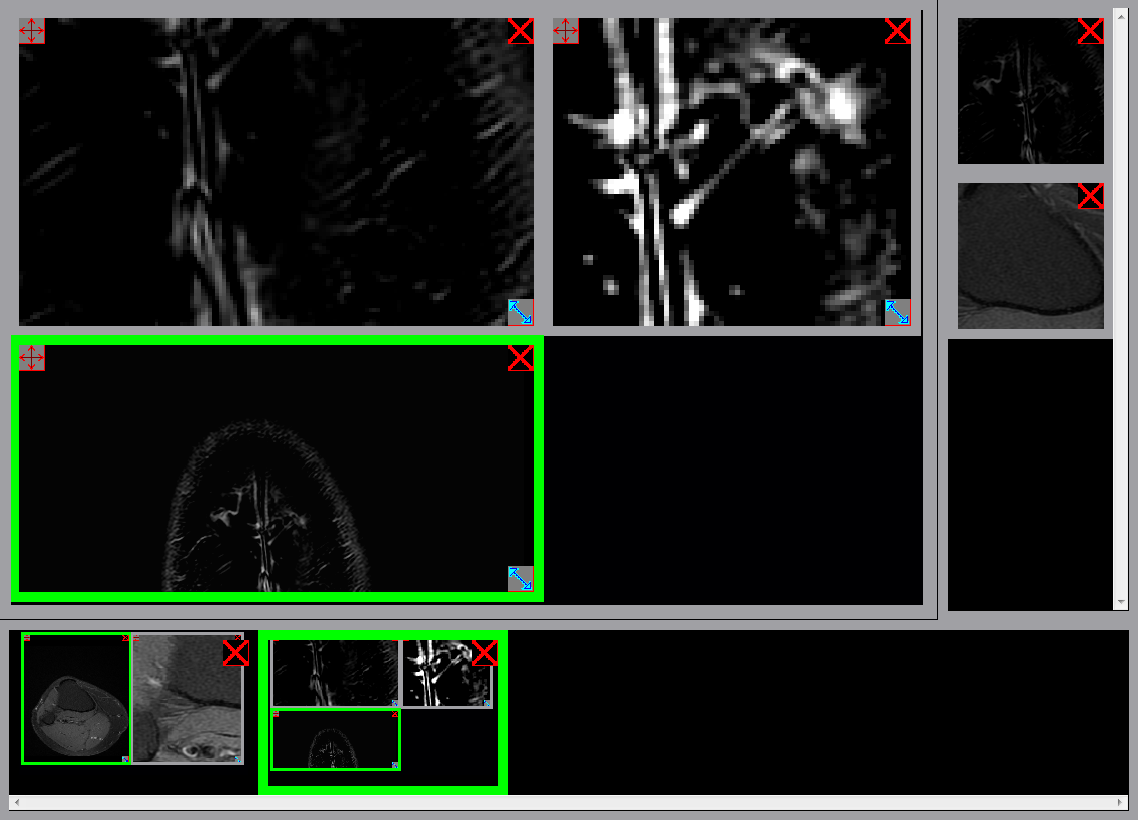
\includegraphics[width=\textwidth]{Text/IMG/dicom-presenter-gui.png}
	\end{center}
	\label{paint}
\end{figure}

\subsection{Graphic Output Rendering in Dicom-Presenter}
The mentioned control elements of Dicom-Presenter: Image Explorer and Workspace Explorer are rendered manually. They are not based on existing Qt library class. Thus, if a graphic output of Dicom-Presenter is rendered all classes representing some graphic element must be called. 

An impulse to render the graphic window can be called at any time from any part of the application. A static function is used to obtain the pointer to output window, then a function called \clist{paint} is called.

The \clist{paint} function of main window object (\clist{CWidget}) then calls paint functions of all elements present in the window: an active Workspace, Workspace Explorer and Image Explorer. All the elements contain smaller subelements. The Workspace calls paint functions of all images present appearing on the Workspace, Workspace Explorer calls paint functions of all images containing workspace previews and finally the Image Explorer calls paint functions of all images operated by it. A schema of the process can be seen on Figure \ref{paint}.

\begin{lstlisting}[label=cwidgetpaint,caption={Sequentionally rendering each visible element.},escapeinside={@}{@}]
void CWidget::paint() {
	...
	CWorkspaceManager::GetInstance()->GetActiveWorkspace()->paint(...);
	CImageExplorer::GetInstance()->paint(...);
	CWorkspaceExplorer::GetInstance()->paint(...);
	...
}
void CWorkspace::paint(...) {
	...
	while (images.hasNext()) {
	  ...
		cimage->paint(...);
		...
	}
	...
}
void CImageExplorer::paint(...) {
	...
	while (images.hasNext()) {
		...
		cimage->paint(...);
		...
	}
	...
}
void CWorkspaceExplorer::paint(...) {
	...
	while (workspaces.hasNext()) {
		...
		snap.paint(painter);
		...
	}
	...
}
\end{lstlisting}

\begin{figure}
	\caption{A hierarchy of classes presenting paintable elements.}
	\begin{center}
	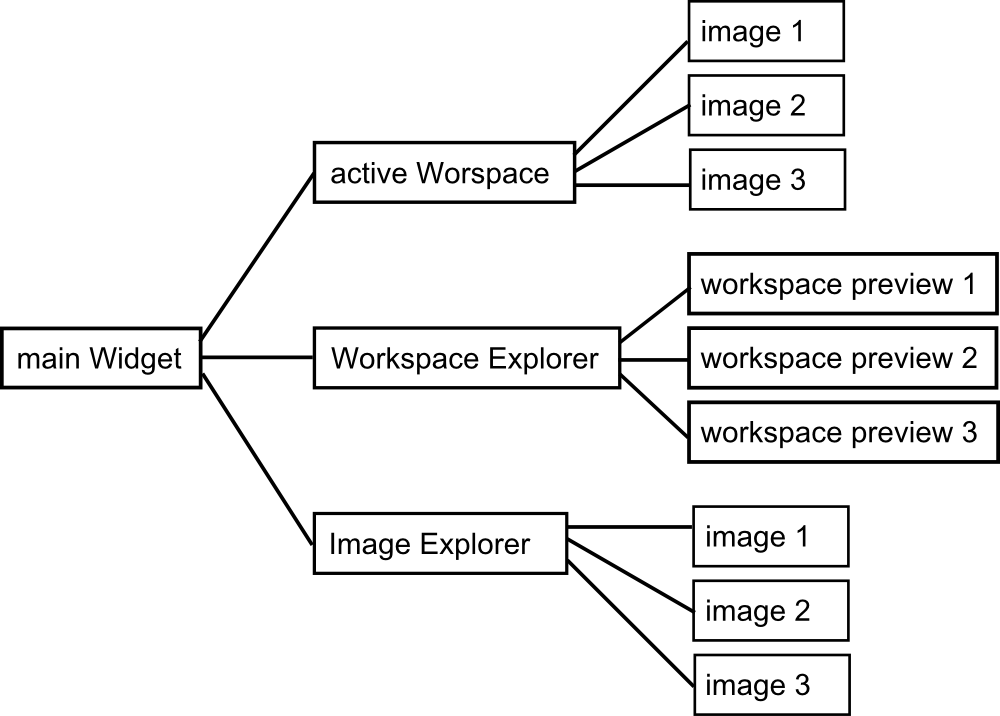
\includegraphics[width=\textwidth]{Text/IMG/paint.png}
	\end{center}
	\label{paint}
\end{figure}

\subsection{Control Event Forwarding in Dicom-Presenter}

Similarly as the paint directions are distributed to the application classes, pointing device events are distributed through the object model. As was said in previous section, all the visible elements of Dicom-Presenter visual output are rendered manually. Therefore, if the user performs some pointing device action on some visible element (wheel-scroll, mouse-click, etc.), the event must be manually forwarded to the related object.

Pointing device events in Dicom-Presenter can be divided into two groups: events starting an action and events related to a previously started action. Mouse click and mouse double click start an action, mouse move and wheel scroll are related to previous event. If a click or double-click event is captured, then the process of finding the related object must be started. If a mouse move or wheel scroll are received, the event is instantly forwarded to the last used object.

The process of finding the object related to click or double-click event is similar to the painting process. The main widget receives a click event together with the position of the mouse pointer in coordinates related to the widget. Each of all three parent elements on the widget (Workspace, Workspace Explorer and Image Explorer) have saved their position in the main widget. Therefore, the main widget asks all three elements if the mouse pointer position corresponds with their position. The element giving positive response receives the event.

If the active Workspace receives the event, then it must be decided which of the opened images is related to the action. Thus, all displayed images are iteratively asked whether their location cover the pointer position. Then, the event is forwarded to the prospective image. The image object performs required task such as move, zoom or brightness change.

Similarly, if the mouse pointer was not located on the active Workspace but on the Workspace Explorer or the Image Explorer, then, the event is redirected to the appropriate object. Afterwards, the object iterates through its owned objects and finds the one related to the event received (workspace preview or image preview). The desired action can be performed.

The schema is different from usual GUI programming techniques where some GUI framework would be used. The framework solves event redirecting itself, as seen in Section \ref{guiframeworks}.

\subsection{Image Opening in Dicom-Presenter}





\section{Rendering Engine Implementation}
\red{podrobne rozepsat, jake tridy byly pouzity a co delaji}
\chapter{Multi-planar Reconstruction}
\vspace{-10mm}
\label{multiplanar}



Multi-planar Reconstruction (MPR) in medical imaging is a method for displaying three-dimensional images, captured on an imaging device. A three-dimensional study is displayed in three orthogonal slices. In each slice, there are indicated positions of the other two slices - each slice includes two lines giving the positions (See Figure \ref{fig:multiplanar}). The slices are most often parallel to basic anatomy planes\cite{ctteachingmanual}: sagittal, coronal and transverse plane.  Implementation of Multi-planar Reconstruction was requested by IKEM.

\begin{figure}
 	\caption{Multi-planar reconstruction in Dicom-Presenter.\label{fig:multiplanar}}
	\begin{center}
	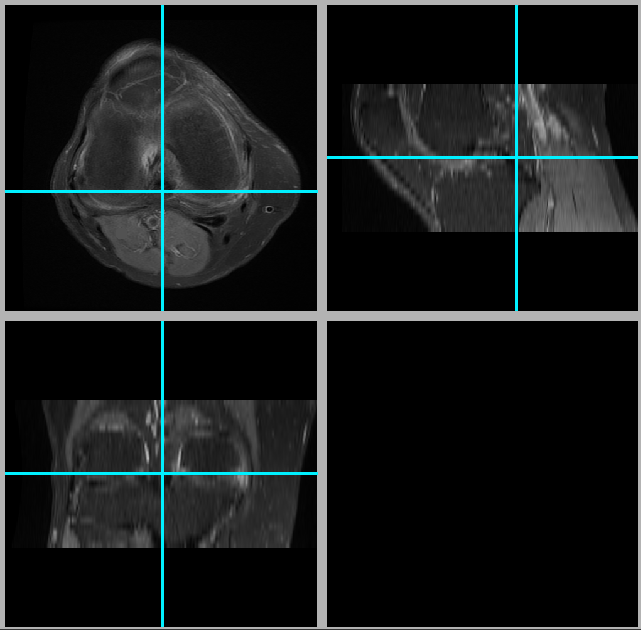
\includegraphics[width=0.75\textwidth]{Text/IMG/MultiPlanar.png}
	\end{center}
\end{figure}

\section{Designing an Object Model of Multi-planar Reconstruction}

An implementation of MPR could be divided into three parts:

\begin{itemize}
\item Handling user control.
\item Image Rendering.
\item Integration to existing object model. 
\end{itemize}

The question to discuss in all three steps is, how much of the existing functionality can be used and what parts are necessary to be implemented. It is possible to implement a completely new class, which will handle user control and rendering itself. But this would lead to multiple implementations of similar tasks. The aim is to use the maximum possible amount of existing functionality.

The functionality of new classes performing Multi-planar reconstruction will be similar to existing classes: Workspace and Image. Workspace class manages placement of images on the computer screen - similarly, three slices of MPR will be placed on computer screen. There is a process of obtaining the appropriate slice from a three-dimensional image in the Image class. When using MPR, three slices will be taken in three orthogonal planes.

The similarities to Image and Workspace classes could be solved in several possible ways:

\begin{itemize}
\item It is possible to create a new standalone class, which will have partially similar functionality to the existing one.
\item The new functionality can be added to the existing class.
\item The existing class can be inherited by the new class.
\item An identical functionality of the class and existing class can be extracted into an abstract class, which will be inherited by both of them.
\end{itemize}

The most importance was given to the fourth option, because unlike the first option it does not add source code repetition. In addition it does not lead to creating classes with great volume of rarely used source code unlike the second option.

\section{Implementation Process of Multi-planar Reconstruction}

The class of Multi-planar Reconstruction (further MPR Workspace class), which will hold simillar function as the Workspace, was implemented as a new standalone class. The class has firmly defined layout of including images and respones to mouse events are re-defined. The MPR class owns one object of Image type. New functions for MPR rendering were added to the existing Image class.

This solution is fully functional, but it has two disadvanteges:

\begin{itemize}
\item Firsly, the MPR functions added to the Image class were constantly unused outside MPR.
\item Secondly, a relation between a Workspace and Images is different to relation between MPR Workspace and displayed Images. The MPR Workspace includes one Image object, which is responsible for rendering all three slices. More reasonable solution would be, that MPR Workspace would own three Image objects, each of them responsible for rendering one slice. This scheme corresponds to previous understandings of Image and Workspace. But moreover it would allow the three slices to by fully adjustable like an ordinary Image object (position, size, zoom, ...). 
\end{itemize}

To remove the first complaint, it will be needed to add the MPR functions to a new class and inherit the existing Image class. To avoid the second disadvantage, it will be needed to change the object design of MPR:

\begin{itemize}
\item The responsibilities of processing the user input will be shifted from the MPR Workspace class to the Image class.
%\item Then, it will be possible to allow moving and resizing the MPR Images along the Workspace easily\footnote{The Image position will be bound to the Image GUI.}.
\item The next step will be creating an abstract class describing the positions of all three slices.
\item Afterwards, three Image classes will be used for rendering the MPR. Then, the images will be fully accessible for manipulation.
\end{itemize}




\chapter{Project build environment}
\vspace{-10mm}

Dicom-Presenter is a large application. It consists of 5.000 source-code lines and it uses six external libraries. Therefore, it is not easy to compile it. Compilation of such a large project should be divided into parts, then a linking process should be described somehow. Moreover, external libraries have to be compiled in a compatible configuration. This chapter's goal is to describe compilation process of larger projects.

\section{Libraries}

\label{library}

A C++ application usually isn't compiled all in one step. It is divided into smaller logic parts usually called libraries. These libraries are compiled individually and then they are linked into the executable at the end. The benefit is that if the source code of the application is changed it is not needed to recompile the whole application. While, only the library including the change is recompiled. 

There are two ways of linking a library into a final executable: static linking and dymanic linking.
\begin{itemize}
\item Static linking of a library means that all function of the library are copied into the executable. Firstly, a library's source code is compiled into a .lib file and then it is inserted as a whole into the executable file.
\item Dynamic linking of a library means that only the library's name and its function names are inserted into the executable. An executable code of the linked library is distributed together with the executable file in a standalone .dll file. When the application is ran the operating system has to load library's executable code into the application's virtual memory. While compiling a dynamic-link library the compiler produces also a .lib file. The executable is linked against this .lib file but the lib file contains only instructions to load machine code from .dll files.
\end{itemize}

In addition, there is one more way how to use dynamic-link libraries:

\begin{itemize}
\item Dynamic-link libraries can be also loaded manually during the application run. Windows API offers a set of functions for run-time loading functions from .dll libraries. This is useful for rarely used functions. They don't need to occupy memory space all the time an application is ran.
\end{itemize}

A concept of dynamic-link libraries shows its potential when applied on libraries which are used by multiple applications. Dynamic-link libraries are also called shared libraries. These are the advantages of using shared libraries:

\begin{itemize}
\item If a dynamic-link library is used by multiple applications it is enough to be loaded once in computer memory. Multiple applications can access library functions at the same time.
\item If a library needs to be updated, there's no need to recompile the applications using library as far as library's function declarations aren't changed.
\end{itemize}


\section{Run-time loaded libraries}

\red{
Co to znamena run-time loaded library?\\
Proc potrebujeme run-time loaded library? No kvuli pluginum.\\
}

\subsection{Compilation of run-time loaded libraries}


A run-time loaded \clist{.dll} library is very similar to an \clist{.exe} binary, but there is a function exports table in a \clist{.dll} library. Exported functions are accessible from outside of the library, functions not exported are private functions. Therefore, a compiler needs to know which functions have to be exported. There are two ways for declaring this: a \clist{dllexport} macro can be used or a \clist{Module Definition File} can be used. A \clist{Module Definition File} is a file including a list of exported functions using a very simple syntax. There is an example of a \clist{Module Definition File} in Listing \ref{DEF}. An example of using the \clist{dllexport} macro can be seen in Listing \ref{dllspec}. Placing the macro before a function definition is enough to tell a compiler to export the function.

\begin{lstlisting}[label=DEF,caption={A \clist{Module Definition File} of a library called ``Mathfuncs'' including a function called ``PrimeTest''.}]
LIBRARY   MATHFUNCS
EXPORTS
   PrimeTest	@1
\end{lstlisting}


\begin{lstlisting}[label=dllspec,caption={An example of exporting a function by using a \clist{dllexport} macro.},escapeinside={@}{@}]
#include <iostream>
#include <cmath>
#include "mathfuncs.h"

extern "C"{
	__declspec(dllexport) bool PrimeTest(int n){
	bool isPrime=true;
	for (int d=2;d<=sqrt((float)n);d++){
		if (n%d==0) isPrime=false;
	}
	return isPrime;
}
\end{lstlisting}

\subsection{Run-time loading process}

\label{sec:runtimeloading}

\begin{lstlisting}[label=WinAPI,caption={An application loading a .dll library at runtime.},escapeinside={@}{@}]
#include <iostream>
#include <windows.h>

typedef bool PrimeTestFunction(int);

int main (){
	HINSTANCE LoadedLibrary;
	LoadedLibrary=LoadLibrary(TEXT("MathFuncs.dll"));
	if (LoadedLibrary!=NULL){
		FARPROC ProcessAdress;
		ProcessAdress=GetProcAddress(LoadedLibrary,"PrimeTest");
		PrimeTestFunction* _PrimeTestFunction=(PrimeTestFunction*)ProcessAdress;
		if(_PrimeTestFunction){
			std::cout << "23 is prime number:" << _PrimeTestFunction(23) << std::endl;
		}
		FreeLibrary(LoadedLibrary);
	}
}
\end{lstlisting}



\section{C++ Standard Library in MS Visual Studio}

\label{standardlibrary}
C++ Standard Library\footnote{C++ Standard library is a C++ version of C Run-time library. Unfortunately both names are often confused.} is used in almost all C++ application. It provides communication with the operation system. It offers manipulation with standard input and output (stdio.h), memory allocation (stdlib.h), math functions (math.h), time related funtions (time.h), etc. If the library is used in application its header files are included in source code and the library is linked into executable file.

There are four different implementations of C++ Standard library in Microsoft Visual Studio compiler. The rule is that only one type of implementation can be linked into executable file. The problem is if multiple external libraries are used in one project. Every external library is compiled with use of some kind of Standard C++ library implementation. If we try to link an application against external libraries using different implementations of C++ Standard library we receive a linker error 2005 - already defined. This error arises because multiple versions of C++ Standard library are linked at the same time but they define the same functions.

Therefore, it is mandatory to distinguish implementations of C++ Standard library. All external libraries as well as all inner libraries has to be linked against the same version of C++ Standard library! Standard C++ library implementations differ according to use of dynamic or static linking and according to debug or release building. So, all used libraries has to use static or dynamic linking and all of them has to be builded in debug or release mode. Then, the final application can be linked. Therefore, if we use external libraries we often have to rebuild them to gain proper version of the library using required version of C++ Runtime library.

In addition to the problem explanation the Table \ref{standardlibrarytable} is included. It should help to resolve the purpose of problem when receiving linker eror 2005. 

\begin{table}
  \caption{A list of four build configurations using different implementation of C++ Standard Library.}
  \label{standardlibrarytable}
	\begin{tabular}{| l| l | l |}
	  \hline                       
	  Link type & Build mode & Library file \\
	  \hline
	  \hline                     
	  Static & Debug & LIBCPMTD.LIB\\
	  \hline
	  Static & Release & LIBCPMTD.LIB\\
	  \hline  
	  Dynamic & Debug & MSVCPRTD.LIB\\
	  \hline  
	  Dynamic & Release & MSVCPRT.LIB\\  
	  \hline  
	\end{tabular}
\end{table}


\section{CMake}


As mentioned before, C++ projects are usually compiled in parts and then linked together at the end. So, the build process has to be described somehow. The description includes mainly information about:

\begin{itemize}
\item Grouping project files into project libraries.
\item Dependency on external libraries.
\item Description of custom build steps.
\end{itemize}

Microsoft Visual Studio uses its own format of build description accessible from its GUI. There is GNU Automake system for build decription on Unix systems. Since Dicom-Presenter was supposed to be a multi-platform application there was a need to find some system of build description applicable on both Windows and Unix systems. A reasonable solution is a use of CMake, because offers a platform-independent build description. CMake script describes a build tree as well as project dependencies. Then a CMake tool offers generating Visual Studio project for Windows OS or GNU automake files for Unix OS.

CMake is often use in OpenSource projects. It offers easy portability of an application between Win32 and Unix based systems. Both plib and dcmtk libraries used in Dicom-Presenter use CMake for build scripts generation. According to Section \ref{standardlibrary} both libraries needs to be compiled before compiling Dicom-Presenter.

\subsection{CMake syntax}


Following section describes CMake syntax necessary to build simple applications. 

A CMake build description is always written in a file named \clist{CMakeLists.txt} and placed in project root directory. At the beginning of the file there has to be preamble requesting CMake of newer version than declared: \clist{cmake\-\_minimum\-\_required\-(VERSION ...)}.

When compiling from a command line with use of gcc or g++ it is necessary to mention where can compiler find header files from external libraries and where can linker find .lib files from external libraries. CMake uses commands \texttt{include\-\_directories\-("...")} and \texttt{link\-\_directories\-("...")} for defining paths to libraries.

As mentioned in Section \ref{library}, C++ applications are firstly compiled in parts into internal libraries and then linked together. A library compilation is in CMake declared by command \texttt{add\-\_library\-(library1 library1.cpp library1.h ...)}. The first parameter is a name of the library. It is the name of the output file, but moreover it is the name under which CMake remembers this library. The other parameters make a list of files which will be compiled as the library.

If a library depends on external libraries a command \texttt{target\-\_link\-\_libraries\-(library1 lib1 lib2)} defines the dependencies. The first parameter is the name of the internal library. The other parameters are filenames of external libraries.

It is possible to add custom build commands with statement: {\tt add\-\_custom\-\_command\-(COMMAND command1 OUTPUT outputfile1)}. A shell command follows a \clist{COMMAND} macro. It can by any Linux or Windows console command including a program call. The second argument placed after \clist{OUTPUT} macro is a label for an output file generated by the command. Then, this file can be used for building later in CMake script. It can be a source-code file, resource file, library, etc.




\definecolor{LightGray}{RGB}{245,245,245}
\definecolor{LightRed}{RGB}{150,150,150}
\definecolor{LightGreen}{RGB}{0,0,0}
\definecolor{LightBlue}{RGB}{100,100,100}
\lstset{ %
language=C++,                % choose the language of the code
basicstyle=\tt\small\color{LightBlue},          % print whole listing small
keywordstyle=\small\color{black},	% bold black keywords
identifierstyle=\small\color{LightBlue},           % nothing happens
commentstyle=\small\color{Rhodamine}, % white comments
stringstyle=\ttfamily,      % typewriter type for strings
showstringspaces=false,     % no special string spaces
numbers=left,                   % where to put the line-numbers
numberstyle=\tiny\tt,      % the size of the fonts that are used for the line-numbers
%stepnumber=2,                   % the step between two line-numbers. If it's 1 each line will be numbered
numbersep=5pt,                  % how far the line-numbers are from the code
%backgroundcolor=\color{LightGray},  % choose the background color. You must add \usepackage{color}
showspaces=false,               % show spaces adding particular underscores
showstringspaces=false,         % underline spaces within strings
showtabs=false,                 % show tabs within strings adding particular underscores
frame=single,			% adds a frame around the code
tabsize=3,	                % sets default tabsize to 2 spaces
%captionpos=b,                   % sets the caption-position to bottom
breaklines=true,                % sets automatic line breaking
breakatwhitespace=false,        % sets if automatic breaks should only happen at whitespace
%title={Zdrojovy kod},                 % show the filename of files included with \lstinputlisting; also try caption instead of title
%escapeinside={\%*}{*)}          % if you want to add a comment within your code
escapechar=!,
}

\begin{lstlisting}[caption={Skript systému Cmake pro překlad programu Dicom Presenter}, language=make, morekeywords={cmake_minimum_required, project, set, include_directories, link_directories, add_custom_command, OUTPUT, COMMAND, add_library, target_link_libraries, ADD_EXECUTABLE},keywordstyle=\small\color{LightGreen}]
cmake_minimum_required(VERSION 2.8)
project (dicom-presenter)

set (Qt_LIBRARY_PATH /usr/share/qt4)
set (Cg_LIBRARY_PATH /usr)
...

include_directories (!\redlist{``./src''}!)
include_directories (!\redlist{``\${Qt\_LIBRARY\_PATH}/include''}!)
include_directories (!\redlist{``\${Cg\_LIBRARY\_PATH}/include''}!)
...

link_directories (!\redlist{``\${Qt\_LIBRARY\_PATH}/lib''}!)
link_directories (!\redlist{``\${Cg\_LIBRARY\_PATH}/lib''}!)
...

add_custom_command (OUTPUT moc/moc_mainWindow.cpp COMMAND moc src/mainWindow.h > moc/moc_mainWindow.cpp)
add_library (mainWindow src/mainWindow.cpp moc/moc_mainWindow.cpp src/mainWindow.h)
target_link_libraries (mainWindow QtGui GLEW)

add_library (glImage src/glObjects/glImage.cpp src/glObjects/glImage.h)
target_link_libraries (glImage QtOpenGL QtCore)

...

ADD_EXECUTABLE (dp src/main.cpp)
target_link_libraries (dicom-presenter mainWindow glImage ...)
\end{lstlisting}




\chapter{Plugin system}
\vspace{-10mm}

There was a need of image segmentation support in Dicom-Presenter. A few of FNSPE student are working on image segmentation algorhitms of MRI images. Therefore raised an idea to import these algorhitms into Dicom-Presenter. The best idea was to design a plugin system for importing segmentation algorhitms.

Plugin in computer sciences is an optional addition to some application. It is not usually distributed with application itself, but can be added by user according to his needs. An example of a plugin can be an additional python script to Gimp program which allows user to apply 'sepia effect' on his photos. According to the mentioned example, plugins can be written in another language than application itself. They obtain some new functionality to application.

All segmentation algorithms developed at FNSPE were written in C language due to its performance. Plugins in C language are compiled to a Dynamic-Link libraries and run-time loaded. A theory of C++ libraries and description of run-time loading libraries can be found in Section \ref{library}.

\section{Image segmentation algorithms}

\red{
Popsat algoritmy Kuby Louckeho a Radka Maci.\\
}

\section{Plugins system requirements}

It is needed to set rules for plugin libraries. Every library following these rules should be automatically usable in DicomPresenter. The first thing is to generalize what the libraries will need as an input and output. All three libraries made by FNSPE students just needed a picture and few parameters as an input. The parameters can be inserted into text fields by a user. Therefore, there has to be an opportunity to generate these text fields dynamically while loading a plugin. A computing algorithm in a library is ran by a function call of some function in the library. This function receives the parameters inserted by the user.

All three algorithms receive input image only as a file path on a disk. Images in Dicom-Presenter which user can see are two-dimensional projections of a three-dimensional picture - they are not stored in a file but just in a memory. Therefore, it will be needed to save them into a file to be processed by a segmentation algorithm.

\red{
Pavel: Pridat informace o tom, ze pozadavky na plugin system byla dale jednoduchost implementace pluginu.\\
Pavel: Pridat zminku o tom, ze algoritmy maji parametry a je potreba umoznit nastavovani techto parametru.\\
}

\section{Generating plugins GUI}

Dicom-Presenter GUI is written with use of Qt framework. GUI elements are created as objects of Qt classes and assigned to existing GUI elements. Dicom-Presenter plugin API has to be prepared for various number of text and numeric input fields. Therefore it is mandatory to pass information about GUI appearance to Dicom-Presenter. The goal of this section is to find the must suitable way of plugin GUI description.

Qt library offers it's own way for GUI description. There's a tool in Qt SDK which offers an interactive GUI creation. It produces a XML file which describes the GUI. A strong argument for using this solution is that Qt library offers its own tools for loading these files.

Another possible way was to declare our own language for plugins GUI description. Firstly it was implemented easily: Lines in a description file were corresponding to GUI elements. First word of a line determined a type of an element. Other words on the line described element behaviour such as default value, minimum and maximum value or a corresponding function in a library. In a second step GUI description was improved according to modern standards and implemented in XML - in a simillar way like in previous case.

It would seem that the first solution is more reasonable. We don't declare some new language but we use an existing standard from Qt library. This is in many cases right way of thinking. Unfortunately the Qt library syntax was primarily supposed to be generated by their tool. Their XML code was too complicated to be written manually - there were too much required phrases in their code. Morover, GUI elements were described by their class-names in Qt library - so it would be needed to know Qt library to write description manually. The only option would be to generate the code by their interactive tool. Unfortunately the tool was still too complex and complicated, aimed to creating extensive GUI layouts for large applications. In our case we need just description of few numeric and text input fields and one or more buttons. It seemed much more easier for a programmer to just follow our few rules for GUI description instead of using Qt library's extensive standard.

As mentioned above, external libraries for image segmentation just need a few numeric input fields for giving computation parameters and then a filename of an input image. For a better flexibility of our plugin solution there were added an option for passing char-type parameters and a possibility to run more functions in a library.

For every numeric input field it is needed to know: a required variable type (integer or float), minimal and maximal possible value, default value, parameter description. Passing char parameters was realised by a combobox element. So it is needed to know all possible values, text description of values and an overall description of the property. 

The language for Dicom-Presenter GUI description is supposed to be simple. A numeric field is declared by a string:

\clist{<numinput type="..." min="..." max="..." default="..." name="..."/>}

Where \clist{type} determines a C/C++ type (integer of double), \clist{min}, \clist{max}, \clist{default} determine minimum, maximum and default value and \clist{name} determines a parameter description.

A combobox can be declared in a similar way like in (X)HTML:

\noindent \indent \clist{<combobox type="..." name="...">}\\
\indent \indent \clist{<option value="..." name="..."/>}\\
\indent \indent \clist{<option value="..." name="..."/>}\\
\indent \clist{</combobox>}

Where \clist{type} determines a variable type passed to a library. \clist{name} in \clist{combobox} tag is a text description of property. The \clist{name} property in \clist{option} tag is a text description of a \clist{value} which is passed to a library.


\begin{comment}
First idea was to use our own way to describe plugin GUI. The first version of plugins system used it's own primitive language. Lines in description file were corresponding to GUI elements. First word of a line determined a type of an element. Other words on the line described element behaviour such as default value, minimum and maximum value or a corresponding function in a library. This own language of GUI description was sufficient but it was unnecessary to force plugin programmer to use our own language. Instead it would be better to use some existing standard.

Other way how to describe a plugin GUI was to use XML language. XML is often use in computer science to pass information in an easily processable form. Moreover Qt library includes extended tools for XML processing.

Last option is to use Qt language for UI description. Qt library uses it's own form to describe application GUI - description is in a special file with a \clist{.ui} extension. It is a strong argument for this option that it is a native way for Qt library to use this langage. Qt library provides a utility for interactive GUI creating. 
\end{comment}



\section{Dynamically loading plugin functions}

Dicom-Presenter plugins can use different number of parameters. A C/C++ function from dynamically loaded library is ran through a pointer to the function as we saw in \ref{sec:runtimeloading}. This pointer must have a fixed number and fixed types of parameters given at compiliation. Thus, it is not possible to call any function which needs any set of parameters from a dynamically loaded library. It is possible to run only a finite number of types of functions according to a set of given parameters. There were several solutions how to make the Dicom-Presenter plugin system variable enough to load and run various functions:

\begin{enumerate}
\item It is possible to try to define sufficient number of function pointer types at a compilation time. Then set a rule that every Dicom-Presenter plugin can have input function only of predefined type.
\item Another solution is based on a fact that a function pointer can have more parameters than targeted function. For example a function pointer having five integer parameters can point to a function receiving only three integer parameters - the last two given parameters will be ignored. Therefore it would be possible to define function pointers with excessing number of float, integer and char parameters. A function pointer would be assigned to a function to fit with the first couple of parameters ignoring the rest.
\item Another way which seems applicable but still presuming too much conditions from a loaded plugin was too allow only one-parameter functions in the plugin. These functions would set parameters in a library as global variables. Before running a computation all functions setting some parameter would be ran. This solution has a great advantage: It is possible to call the functions to set parameters right when user is manipulating with relevant GUI elements. So, there can be a feedback from the library telling user he set some incompatible set of values. This solution was implemented at first but it seemed too restrictive for a library design. 
\item Last option is inspired by an obligatory passing command line arguments to a standard C/C++ application. C/C++ Main Function receives a pointer to an array of all arguments. As in this case a plugin library function can receive three pointers to three array types: pointer to int, pointer to double and pointer to char. The arrays can be of any length.
\end{enumerate}

At first the third option was used in implementation (See an example on encloced CD). Function setting algorithm parameters were called while setting parameters in GUI. But there were no real benefits of a library response while setting GUI parameters. More than that the rules for plugins were too bounding. So therefore, the final version of plugins API were implemented using option 4.

\section{User Interaction in Image Segmentation plugins}

\red{
Popsat jak uzivatel musi nakreslit seminku krivky.\\
Popsat implementaci, jaka byla pouzita.\\
}
%%%%%%%%%%%%%%%%%%%%%%  LITERATURA  %%%%%%%%%%%%%%%%%%%%%%

\nocite{*}				% zobrazuj i necitovane primarni zdroje
\bibliography{Text/Literature}
\nocitesec{*}				% sek. zdroje
\bibliographysec{Text/Sec}


\end{document}
